 \section{Results}\label{sec:results}
We collected data for the first hour of every day of April 2017. This resulted in just over 700,000 BGP announcements. We found 21 incidents labeled as  `hijacks or misconfigurations. We identified 3 international organizations, with ASes in different countries. We found that the hijacked prefixes belonged to China, Pakistan and Bangladesh. They were falsely announced as having AS origins in Vietnam, India and India, respectively.
Here we highlight various aspects of our results. 
\subsection{Types of origin AS conflicts}
Figure~\ref{fig:conflict_source} gives an indication of the proportion of different types of prefix origin AS conflicts . We do not interpret this result as being exact but as an estimate for the proportions of each type of conflict. In addition, we reemphasize that each level is exclusive of the conflict incidents occurring in the others.
 \begin{figure}
	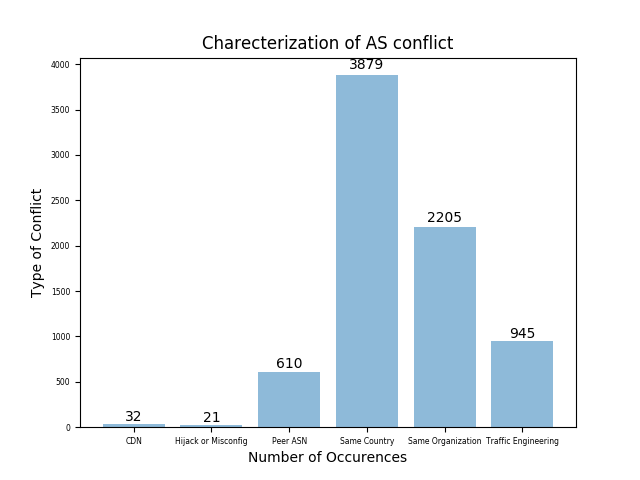
\includegraphics[width=0.5\textwidth]{AS_Origin_Conflict_Types.png}
	\caption{Bar graph shows the number of incidents for each source of prefix origin conflict.}
	\label{fig:conflict_source}
\end{figure}
`Same country' has the highest number of occurences followed by `same organization' then `traffic engineering'. As indicated by the occurrence of `hijack or misconfig' label, our algorithm is able to greatly narrow down the list of potential hijacks. 
\subsection{Hijack Duration}
The duration of hijack and/or misconfiguration ranged from a few minutes to 13 hours. We expect the hijacks lasting more than a few hours to be outliers or misclassification. There were quite a few outliers, hence we choose to report median hijack duration which was 1367s, roughly equivalent to 23 minutes. 
\subsection{Location}
 \begin{figure}
	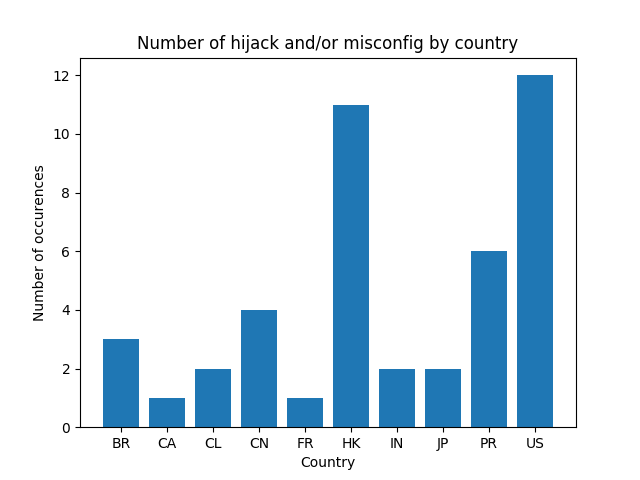
\includegraphics[width=0.5\textwidth]{Occurences_by_country_2.png}
	\caption{Bar graph shows the number of incidents labeled `hijack or misconfig' for 10 most common countries on April 1st.}
	\label{fig:conflict_country}
\end{figure}
Figure~\ref{fig:conflict_country} shows distribution of `hijack or misconfig' for a day's worth of data in April. The graph for the first hour of each month for April shows similar pattern with US showing the largest number of occurrences. In addition, countries such as Vietnam and Australia also occur when we consider only the first hour of each day in April. 
\subsection{Common destinations and attackers}
We found  a wide range of destinations labeled as `hijack or misconfig'. Some incidents were Yahoo Japan Corporation's prefix briefly taken over by `ULKT-AS',  AZUKI LLC's prefix taken over by 'GATEWAY INC'. 

It is important to note that misconfigurations are potentially unconfirmed hijackings. We found some interesting patterns in the misconfigurations of specific countries. Most of the Australian misconfigurations had the AS origin 4739. The United States announced incorrect ASes for prefixes spanning several continents, including Europe, Asia and Africa. We found that most of the misconfigurations announced by Vietnam, had prefixes owned by China. 

We also see a lot of conflicting announcement for traffic engineering purposes. One AS belonging to an organization would announce more specific prefix compared to the other AS of the same organization. We ignored conflicts spanning multiple neighboring countries. For example, there were several alerts of conflicts in which AS-origins were in Colombia and Brazil, or Hong Kong and China. We did not label these as conflicts, and filtered them out manually.

